% 
%   How I want to get to the Solution and why I choosed it also how it works.
%   Also there should be some theory about state estimation and the kalmanfilter used
%   in this
%   
%   \section{Tipps/Notes}
%   - Don't forget point of origin / reference system

  
  \section{Verification}
  First of all the test concept has to be defined on which the developed algorithms will be tested.
  This is also be specially useful for the future competitions to test the adjusted state estimator which are used there.
  For this the following concept figure \ref{fig:Verification} was developed.
  
  \begin{figure}[h!]
   \centering
   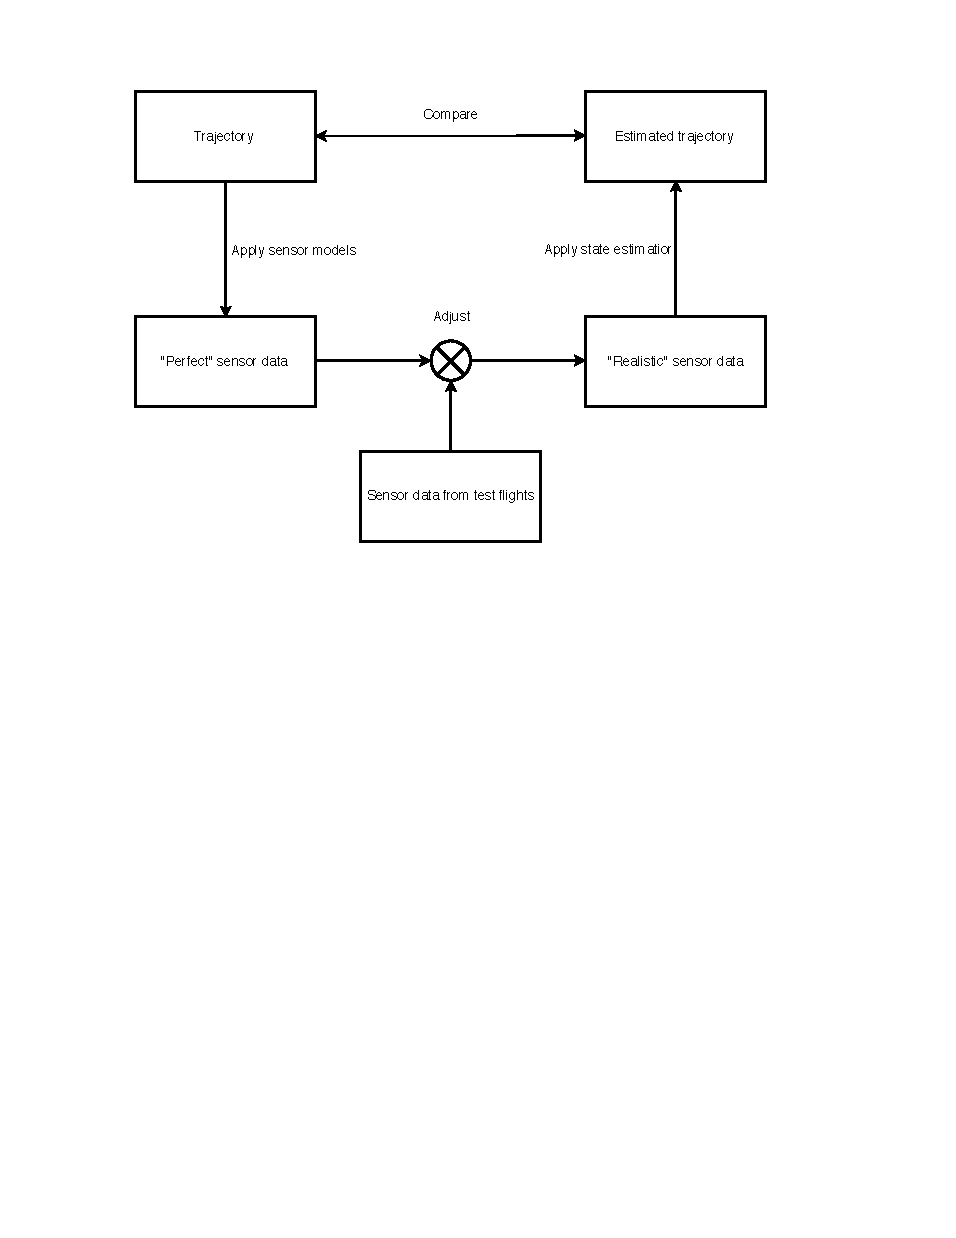
\includegraphics[width = \textwidth]{../BDADoku/Pictures/Verification.pdf}
   \caption{Verification Concept}
   \label{fig:Verification}
  \end{figure}

  The theory behind this is that a trajectory is generated by the simulation, which should resemble a real trajectory as good as possible.
  This function was provided by the simulation team of ARIS from the last years competition.
  Then this trajectory is applied on the sensor models which are developed in chapter \ref{ch:Implementation}.
  This generates so called perfect sensor data. 
  After this the noise is applied which will also be developed later in this chapter, which will result in real sensor data. 
  This noise is drawn out of the sensor log data from the previous test flights.
  After the realistic sensor data is generated, it serves as the input to the different estimation algorithms.
  
  Then to verify the functionality of those algorithms, the estimated trajectory is then compared against the generated trajectory.
  
  
  \section{Sensor models}
  As stated above the trajectory will be generated by the simulation. 
  This are just the information of the height, so the different sensor models have to be adjusted to get to the different needed data.
  The models are defined as follow.
  
  \subsection{Accelerometer}
  Perfect measuring from the accelerometer is in simple terms the two times deviation of the height.
  $$a = \frac{d^2h}{dt^2}$$
  This equals in the straight up acceleration. To get the acceleration which would be provided by an accelerometer,
  the pitch angle has to be calculated into this generated data.
  
  \subsection{Gyrometer}
  For the gyrometer there does not really exist a model with which those measurements could be generated.
  Therefore it has to be generated free hand by taking the gyrometer measurements from the testflights into account.
  It has also to be sayed that only the pitch angle of the rocket which can be seen in figure \ref{fig:RocketPitchAngle} is for interest for this first sensor fusion implementation,
  So only this angle will be generated
  
  \begin{figure}[h!]
    \centering
    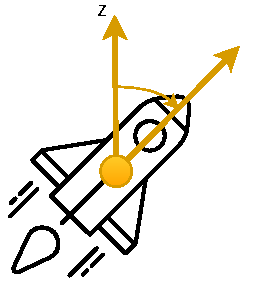
\includegraphics[width = 0.3\textwidth]{./Pictures/RocketSyMod.pdf}
    % RocketSyMod.pdf: 0x0 pixel, 300dpi, 0.00x0.00 cm, bb=
    \caption{Pitch angle visualisation}
    \label{fig:RocketPitchAngle}
  \end{figure}

  
  \subsection{Barometer}
  The barometer which are used in the aerospace usually provide the pressure in hecto Pascal as well as the temperature in degree Celsius.
  \subsubsection{Pressure}
  To generated the pressure data, the barometric height formula is used %Hier Internet Referenz einfügen
  $$P = P0 \cdot (1- \frac{Tgrad\cdot h}{T0})^{\frac{M\cdot g}{R\cdot Tgrad}}$$
  \begin{tabbing}
  with: \= PO = Pressure at ground level \\
  \> TO = Temperature at ground level \\
  \> Tgrad = Temperature gradient for the actual weather condition \\
  \> M = Molar mass of Earth's air: 0.0289644 kg/mol\\
  \> g = Gravitational acceleration: 9.80665 m/$s^2$\\
  \> R = Universal gas constant: 8.3144598 J/mol/K\\
  \end{tabbing}

  This is more or less accurate till 11 000 meter under the condition that the Temperature gradient is determined correct. 

  \subsubsection{Temperature}
  The temperature depending on the height is a difficult subject because the temperature gradient is depending on the actual weather and the capacities of the air.
  So this gradient has to be determined before the start for each flight.

  $$T = T0 - Tgrad*h$$
  
  \subsection{GPS}
  The perfect GPS data is seen as the accurate height but with a slow sample rate around 0.5 to 2 Hz.
  This can simply be achieved by down sampling the height vector with the right factor.
  
  \section{Noise generation}
  To generate the different noises, first the noise from the test flight has to be extracted.
  If done so, a system can be calculated which represents a white noise filter that generates noises
  that has the same spectral power density as original noise. This process is visualised in figure \ref{fig:WhiteNoiseFilter}.
  
  \begin{figure}[h!]
 \centering
 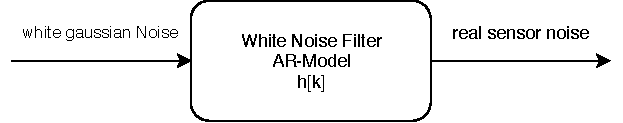
\includegraphics[width=0.5\textwidth]{./Pictures/WhiteNoiseFilter.pdf}
 % WhiteNoiseFilter.pdf: 0x0 pixel, 300dpi, 0.00x0.00 cm, bb=
 \caption{White noise filter concept}
 \label{fig:WhiteNoiseFilter}
\end{figure}
  
  
  For this the yule walker equation should come in handy to calculate a so called AR (auto regressive) model of the noise system.
  An AR model is a FIR (all pole) system which generates a random sequence with defined auto correlation $\gamma_{yy}$ out of white gaussain noise.
  
  $$ y[n] = \omega[n] - \sum_{k=1}^{N} a_k \cdot y[n-k]  $$
  
  The yule walker equations
  \begin{align*}
    \begin{bmatrix}
     \gamma_{yy}[0] & \gamma_{yy}[-1] & \dots & \gamma_{yy}[-N] \\
     \gamma_{yy}[1] & \gamma_{yy}[0] & \dots & \gamma_{yy}[-N+1] \\
     \vdots 		& \vdots 	& 	& \vdots	\\
     \gamma_{yy}[N] & \gamma_{yy}[N-1] & \dots & \gamma_{yy}[0]
    \end{bmatrix}
    & \cdot
    \begin{bmatrix}
     1 \\
     a_1 \\
     \vdots \\
     a_N   
    \end{bmatrix}
    & = 
    \begin{bmatrix}
     \sigma^2_\omega \\
     0 \\
     \vdots \\
     0
    \end{bmatrix}
    \hfill
  \end{align*}
  \hfill
  estimate the coefficient $a_1 \dots a_N $ of the FIR system and the variance of the noise $\sigma^2_\omega $ which can be used to generate a random sequence which has the same auto correlation $\gamma_{yy}$ as the input sequence y.
  Because the AR model consists of an all pole filter, the noise should have has to have a steady mean value preferably it should be zero mean.
  This way the estimated AR model from the yule walker equation can represent the real system at best.
  For this the mean value of the measurements should be calculated beforehand and then be subtracted to get there zero mean noises.
  The part of the mean values that represent noise and can then be added after the noise in generated to represent the real sensors as good as possible.
  
  \section{System Model}
  The system model to represent the rocket will be hold simple to reduce the system load as well as prevent non linearities.
  Also the important values to estimate are at first hand the vertical height and speed, so
  for a first implementation just variables that can bed used do determine those both will be used.
  This are mainly the height and speed from the GPS, the vertical acceleration from the accelerometer
  as well as the pressure and temperature from the pressure sensors. In addition the pitch angle from the gyrometer is used to calculate the pure vertical acceleration.
  But even with such simplification there are different possible system description which have to be taken into account 
  to find the best suitable.
  
  \subsection{General State Space System}
  For this a quick view at general donation of a state space system. First there is the update function.
  $$ \dot{x} = A \cdot x + B \cdot u + G \cdot q$$
  Here the A matrix resambles how the system transmits over time by itself where the B matrix describes how input u does influence the system.
  In addition noise on the system can be described with the G matrix and the noise input q.
  The second equation is the output equation.
  $$ y = C^T \cdot x + D \cdot u + R $$
  Here the $C^T$ matrix describes how the state value from x effect the output while the D matrix describes how input directly effects output.
  The D matrix zero in the most state space systems, because in reality there are not a lot of systems where the output directly and immediately reacts to input.
  Also the noise on the output (measurements) can be described with the R matrix.
  
  \subsection{Point Mass}
  The most simple possible model would be, that the rocket would be resembled as a simple point mass which flies perfectly vertical upwards.
  For this only three state variables would be necessary, the vertical acceleration, the vertical speed and the height.
  $$x = \begin{bmatrix}
  h_z\\
  v_z\\
  a_z
  \end{bmatrix} $$ 
  This would reduce the A matrix of the system to a 3x3 matrix with with only two 1 in it.
   Also the input matrix would be a zero matrix in this system because the input process 
  (power from the motor and drag force from the surrounding air) would be difficult to describe in a linear system.
  \begin{align*}
  A = \begin{bmatrix}
  1 & 0 & 0\\
  0 & 1 & 0\\
  0 & 0 & 0
  \end{bmatrix}
  & \hspace{1cm}
  B = \begin{bmatrix}
          0 \\
          0 \\
          0 \\
  \end{bmatrix}
  \end{align*}
  In addition the measurements which are taken from the sensor will be described as the system output (y vector). 
  So if the pressure from for example two barometers is calculated into the height beforehand it would result in the flowing output matrices.
 \begin{align*}
 y = \begin{bmatrix}
	  h_{GPS}	\\
          h_{p1}	\\
          h_{p2}	\\
          a_z
     \end{bmatrix}
    & \hspace{1cm}
 C^T = \begin{bmatrix}
         1 & 0 & 0	\\
	 1 & 0 & 0	\\
         1 & 0 & 0	\\
         0 & 0 & 1
        \end{bmatrix}     
  \end{align*}
  
  As normal in engineering such a simplification comes with a cost. With this system description the output from the barometer would have
  to be transformed into the height before they could be taken into the system. 
  Due to this the properties of these sensor could not be estimated correct because the value was transformed in a non linear way before it entered the system.
  In addition the same problem occurs with the accelerometer. If the rocket develops a pitch angle not equal to 0 during the asccending, it would be measured wrong.
  To counter this error, the measurements of the accelerometer would have to be weighted with the angle of the gyrometer before entering the system.
  This weighting is also non linear and the values of the gyrometer are not filtered, which would make the estimation even more uncertain.
  
  \subsection{Point Mass with Pressure}
  To taken into account to problem stated above, pressure can be taken into the state vector and therefore be estimated.
  $$ x = \begin{bmatrix}
  h_z\\
  v_z\\
  a_z\\
  p\\
  \end{bmatrix} $$ 
  While this solves the problem stated above, it also produces a new. The system model can only describe linear dependencies between the state variables,
  but the relation between the pressure and the height is clearly non linear in each atmospheric model.
  This dependency can be linearized, but if done so, it does resemble the atmospheric model with less accuracy.
  This linearisation can be used to interpolate between the barometer measurements so the actual pressure is available at any loop iteration.
  This results in a 4x4 A matrix and also a zero B vector for the dynamics equation which look like this:
  \begin{align*}
  A = \begin{bmatrix}
         1    & 0 & 0 & 0    \\
         0    & 1 & 0 & 0    \\
         0    & 0 & 0 & 0    \\
         0    & KP_h & 0 & 0\\
        \end{bmatrix}
        & \hspace{1cm}
    B = \begin{bmatrix}
       0 \\
       0 \\
       0 \\
       0
      \end{bmatrix}
  \end{align*}  
  
  This would also inflect on the output matrices which do then contain the pressure directly.
  In addition the height calculated from the pressure can be inserted as additional measurements to include them into the estimation.
  
  \begin{align*}
   y = \begin{bmatrix}
        h_{GPS}	\\
        h_{p}	\\
        a	\\
        p_1	\\
        p_2	
       \end{bmatrix}
       & \hspace{1cm}
  C^T = \begin{bmatrix}
       1 & 0 & 0 & 0 \\
       1 & 0 & 0 & 0 \\
       0 & 0 & 1 & 0 \\
       0 & 0 & 0 & 1 \\
       0 & 0 & 0 & 1 
      \end{bmatrix}
  \end{align*}
  The input matrix stays the same as above.

  \subsection{Point Mass with Angle and Pressure}
  The same solution as above can also be applied for the pitch angle. 
  But its linearisation is more complicated 
  This would change the state vector from above into the following.
  $$ x = \begin{bmatrix}
  h_z\\
  v_z\\
  a_z\\
  p\\
  \varphi_{pitch}\\
  \end{bmatrix} $$
  This would extend the dynamic part for A into a 5x5 matrix while the B matrix still would be a zero vector.
  \begin{align*}
  A= \begin{bmatrix}
        0 & 1 & 0 & 0 & 0 \\
        0 & 0 & 1 & 0 & 0 \\
        0 & 0 & 0 & 0 & 0 \\
        0 & Kp_h & 0 & 0 & 0 \\
        0 & 0 & 0 & 0 & 0 \\
        \end{bmatrix}
  & \hspace{1cm}
  B = \begin{bmatrix}
             0 \\
             0 \\
             0 \\
             0 \\
             0 \\
        \end{bmatrix}
  \end{align*}
  
  
  %% Maybe do here a beter linearization and put that into here.
  In addition the output matrix and the y vector will also change to adjust for the gyrometer measurements.
  \begin{align*}
   y = \begin{bmatrix}
        h_GPS \\
        h_p \\
        a \\
        p_1\\
        p_2\\
        \varphi_{pitch}
       \end{bmatrix}
       & \hspace{1cm}
       C^T = \begin{bmatrix}
        1 & 0 & 0 & 0 & 0 \\
        1 & 0 & 0 & 0 & 0 \\
        0 & 0 & 1 & 0 & 0 \\
        0 & 0 & 0 & 1 & 0 \\
        0 & 0 & 0 & 1 & 0 \\
        0 & 0 & 0 & 0 & 1 \\
        \end{bmatrix}
  \end{align*}
  This solution would take all measurements available for the needed values into account.
  It would also keep the calculation in the system as simple and linear as possible.
  \subsection{Discretisation}
  The system stated above are all in continuous time state space description. 
  For implementation on a discrete time system like a micro controller they have to be discredited.
  Those discrete matrices which will be denoted with an additional lowercase d (A -> Ad).
  The general state space discrete description with noise looks as follow.
  $$ x[k+1] = Ad\cdot x[k] + Bd\cdot u[k] + Gd\cdot Q[k] $$
  $$ y = C \cdot x[k] + D\cdot u[k] + R[k] $$
  As it can see only the A, B and G matrices have to be discredited this because 
  the matrices used in the second equation are only there for scalar adjustment for the output
  and should there not contain any time depending calculation.
  The Ad matrix can be calculated with the the following formula.
  $$ Ad = e^{A\cdot Td}$$
  Where Ts stands for the sampling time of the system which would be 1 millisecond on the system developed for this thesis.
  In addition there are two known ways to calculate the other needed discrete matrices Bd and Gd.
  \begin{itemize}
   \item $$ Bd = Ad \cdot B $$
	 The first one resembles a perfect sampling which is equal to a multiplication with a dirac impulse.
	 This calculation is rather further from the reality because no sensor can measure with perfect dirac impluse.
	 The great advantage of this method on the other hand is its simple calculation.
   \item $$ Bd = \int_0^{Ts} e^{A\cdot v}\cdot B \ dv $$
	 This version does resemble a zero order hold likewise measurement which is done by most sensors so it is more realistic than the first version.
	 It comes at the cost that the calculation is more difficult \cite{DavidWSchultz2004}.
  \end{itemize}

  Both version have to be tested in the simulation to see if the additional effort for the second version pays of enough.
  
  \section{State estimator}
  There are many possibilities to do sensor fusion. first of all an all new algorithm could be developed which accesses the 
  stated problems directly. While this solution would be preferable regarding the efficency, the 
  time and knowledge needed for this task would exceed the resources given in this thesis by far.
  Also as stated in chapter \ref{ch:Introduction} a lot of theoretical as well as practical pre work is
  already done and therefore should be used. 
  So following different possible approaches with there pro and cons will be discussed. 
  
  \subsection{Kalmanfilter}
  First of all the traditional discrete kalmanfilter has to be discussed as it provides the base for the most known state estimator.
  Its structure provides the optimal estimation of the standard deviation estimation error as long as the noises are Gaussian
  and the observed system can be described by linear differential equations.
  But there lies the problem, a physical system is most often not linear.
  Also the estimated system as well as its variances over the time have to be known to provide this optimal estimation.
  If the noise matrices of the system are static, the filters gain matrices aim for a fix value and can therefore be calculated in beforehand.
  This reduces the computational effort by a significant amount. \cite{DavidWSchultz2004}.
  It should be mentioned that even if the noise is not Gaussian, the kalmanfilter is still the best
  linear estimator as long as the system and its properties are well known \cite{SimonDan2006Ose:}.
  To summarise it, the normal kalman filter is a simple to understand and adjust state estimator in comparison to the following.
  
  \subsection{ROSE}
  The ROSE(rapid ongoing stochastic estimator) is in simple terms three kalman filters in one.
  Where the main filter is used as a normal kalman filter like stated above, the additional two are used to estimated the 
  the system noise as well as the measuring noise. Therefore this sensor preforms better than the traditional kalman filter
  if those noises change over time in a not known fashion and has therefore be estimated.
  Due to this, this sensor needs more computational effort \cite{DavidWSchultz2004}. 
  
  \subsection{Extended Kalmanfilter}
  The extended kalmanfilter provides additional parts to better access nonlinearity in the observed system.
  This by not estimating the state of the system but by estimating the linearized change of the state 
  to the past sate. For this the systems equations have to be derived around the current nominal point in every estimation state.
  This is some sort of Bootstrap solution because the nominal point on which the derivation happens are estimated in the process and
  this estimates are then used to estimate the change between this estimation and the next.
  Therefore the computational effort exceeds even further because each function has to be deviated at each loop iteration \cite{SimonDan2006Ose:}.
  
  \subsection{Unscented Kalmanfilter}
  The unscented kalmanfilter takes the unscented transformation in use to calculate the different interpolating steps.
  The unscented transformation uses a test set of points around the current state and calculates the new values for them using the functions which represent the system.
  Out of these new values calculated from the test set is now the new state estimated by weighting those new values depending on there probability of occuring. 
  With this the state function do not have to be linearized and therefore the the estimation is most time better than that of the extended kalmanfilter.
  But for this the unscented Kalmanfilter needs also to apply the unscented transformation onto the state vectors in each iteration
  and does therefore need even more computational effort \cite{SimonDan2006Ose:}.
  
  \subsection{H$\infty$ filter}
  The H$\infty$ filter is a more diverse approach then the ones described above.
  It was developed to access the problem when the to be observed system especially its noise is not well known.
  In other words it was developed to resemble an as robust as possible state estimator.
  In addition its stability can be easier guaranteed that with a kalman filter.
  For this it consists of additional tuning parameters which makes it more complicated ti use.
  Also in contrast to the kalman filters the H$\infty$ filter minimises the worst-case estimation error 
  in stand of the standard deviation of the estimation error \cite{SimonDan2006Ose:}.
  
  \section{Choosing}
  If the requirements table \ref{tab:Requirements} is taken into the consideration of finding
  the optimal solution, two main requirements occur that define this decision.
  First the system load is a critical requirements and has therefore to be addressed in this process.
  Also for the requirement of modularity the algorithm should be as simple as possible.
  If taken in regard that the system is more or less well known and that the noise can be
  determened with the simulation and the log data from previous test flights,
  a normal kalmanfilter seems to be the most fitting solution.
  This because the performance of the rocket and the sensor should stay the same during
  each flight. 
  
  \subsection{Functioning}
  Since the best fitting state estimator was chose. Its detailed functioning shall be described here.
  This algorithm works in four main equations which can be devided into prediction and correction steps figure \ref{fig:Kalmanfilter}.

  \begin{figure}[h!]
    \centering
    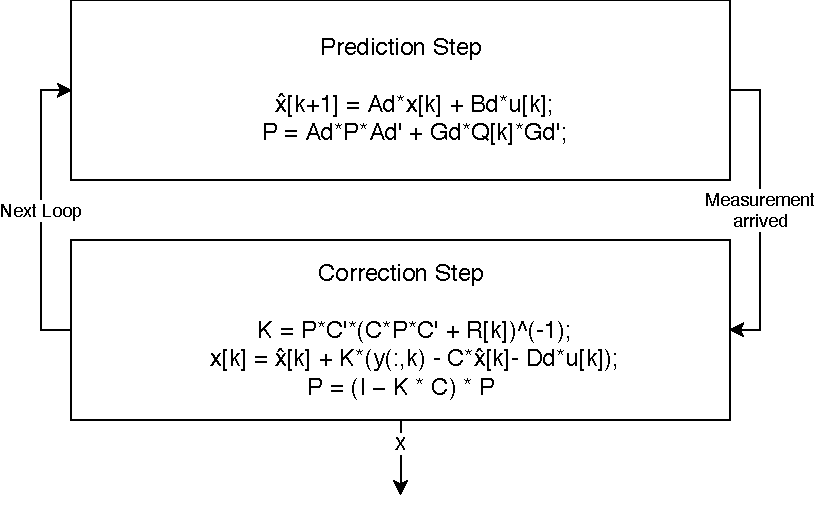
\includegraphics[width = \textwidth]{../BDADoku/Pictures/KalFIlFunc.pdf}
    \caption{Kalmanfilter}
    \label{fig:Kalmanfilter}
  \end{figure}

  \subsubsection{Prediction}
  The prediction equations take the currently values of the state vector ($x[k]$)
  and uses the time depending system model part (A) to predict the state values for the next time step $\hat{x}[k+1]$.
  The hat denotes that this value is an assumption.
  This with the equation: $$ \hat{x}[k+1] = Ad\cdot x[k] + Bd\cdot u[k] $$
  In addition the certainty matrix (P) is calculated which means that it is calculated how trustworthy those predictions are.
  $$ P = Ad\cdot P\cdot Ad^T + Gd\cdot Q[k]\cdot Gd^T$$
  For this the system noise is used, so with the help of the Q matrix it can be stated how well known the system is in this
  time step.

  \subsubsection{Correction Step}
  If the measurements arrive those will be used can be used in the correction step to correct the prediction.
  First the Kalmangain (K) is calculated with the equation.
  $$ K = P\cdot C^T\cdot (C \cdot P \cdot C^T + R[k])^{(-1)} $$ 
  This uses the P matrix from the prediction step as well as the R matrix which represents the measurments noise (how certain the values from the measurements are).
  K is then used in the last equation. $$x[k] = \hat{x}[k] + K\cdot (y[k] - C\cdot \hat{x}[k]-Dd\cdot u[k])$$
  With this the measurement is used to correct the predicted value of the state vector with there uncertainties taken into account \cite{DavidWSchultz2004}. 

  For this the matrices for the system models (A,B,C,D), the measurements noise (Q) as well as the system noises (R) have to be defined.
  
  
  
  